\documentclass[a4paper,12pt]{article}
\usepackage{amsmath}
\usepackage{pdfpages}
\usepackage[utf8]{inputenc}
\usepackage{hyperref}
\usepackage{listings}
\usepackage{xcolor}
\usepackage{calc}
 
\definecolor{codegreen}{rgb}{0,0.6,0}
\definecolor{codegray}{rgb}{0.5,0.5,0.5}
\definecolor{backcolour}{rgb}{0.95,0.95,0.92}

\lstdefinestyle{mystyle}{
    backgroundcolor=\color{backcolour},   
    commentstyle=\color{codegreen},
    keywordstyle=\color{blue},
    numberstyle=\tiny\color{codegray},
    basicstyle=\ttfamily\footnotesize,
    breakatwhitespace=false,         
    breaklines=true,                 
    captionpos=b,                    
    keepspaces=true,                 
    numbers=left,                    
    numbersep=5pt,                  
    showspaces=false,                
    showstringspaces=false,
    showtabs=false,                  
    tabsize=2
}

\lstset{style=mystyle}

\title{Contol theory Homework \#2 report.\\Variant F.}
\author{Anton Brisilin, BS18-02 Student}
\date{\today}
\begin{document}
\maketitle
\section{Task 1.}
\subsection*{A. Calculate total transfer function}
    Calculate total Transfer Function of the system:
    \begin{center}
        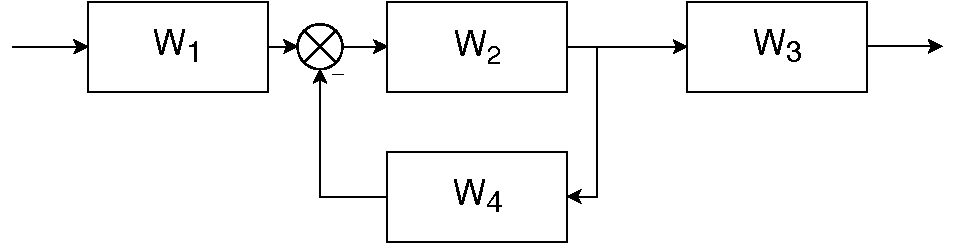
\includegraphics[width=\linewidth/2]{../Task1/ToReport/T1Step0.pdf}
    \end{center}
    As a first step I will simplify feedback chain:
    \begin{center}
        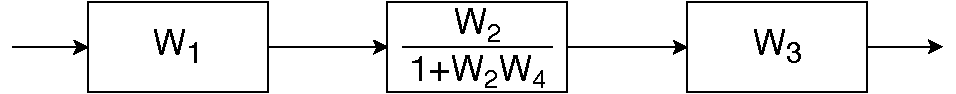
\includegraphics[width=\linewidth/2]{../Task1/ToReport/T1Step1.pdf}
    \end{center}
    And then our system can be represented as one block:
    \begin{center}
        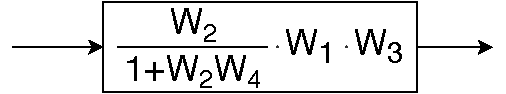
\includegraphics[width=\linewidth/4]{../Task1/ToReport/T1Step2.pdf}
    \end{center}
    In variant F I have:
    \begin{equation*}
    W_1 = \frac{s+3}{s+1}, W_2 = \frac{1}{s+2}, 
    W_3 = \frac{1}{s+0.1}, W_4 = \frac{1}{2s+3}
    \end{equation*}
    Substituting $W_1, ... ,W_4$ to the system block:
    \footnote{This answer was get with Matlab script simplify\_fraction.m in Task1 folder}
    \begin{equation*}
    W_1 * W_3 * \frac{W_2}{1+W2*W4} = 
    \frac{20s^2 + 90s + 90}{20s^4 + 92s^3 + 149s^2 + 84s + 7}
    \end{equation*}
    Hence, our total Transfer Function is 
    \begin{equation}
        W = \frac{20s^2 + 90s + 90}{20s^4 + 92s^3 + 149s^2 + 84s + 7}
    \end{equation}
    \subsection*{B. Build initial and simplified systems and analyse responses}
    \begin{center}
        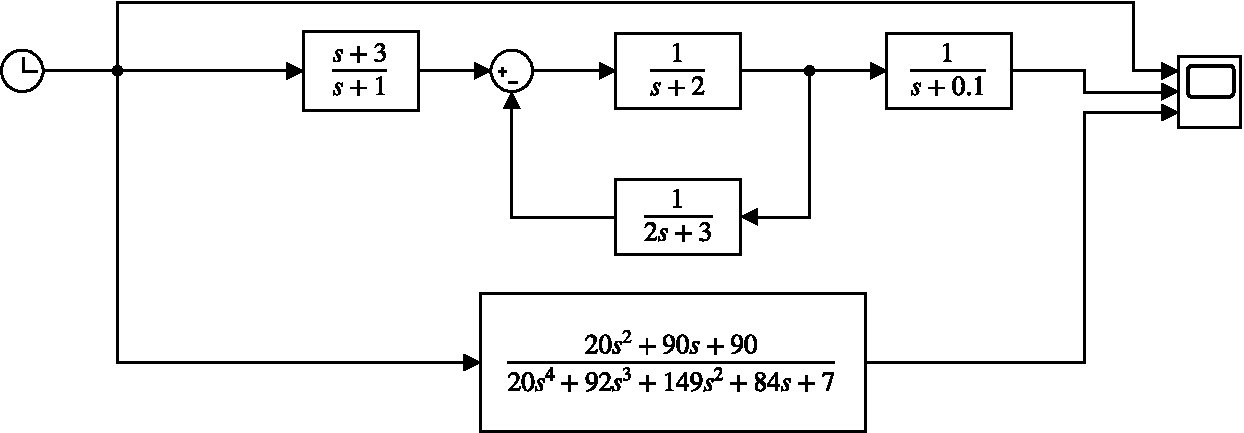
\includegraphics[width=\linewidth]{../Task1/ToReport/T1Model.pdf}
        Simulink model for response analysis. For analysing different responses,
        one just need to put signal source to input instead of the clock.
    \end{center}
    Step, Impulse, and Frequency responses plots. On each plot blue line is 
    system input, red one is the initial system output, and the orange one is
    system output after simplification:\\
    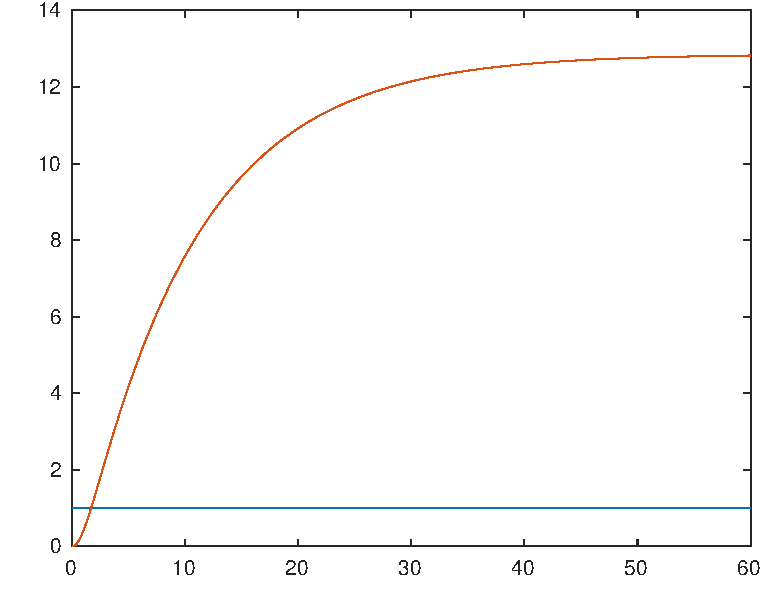
\includegraphics[width=\linewidth/2]{../Task1/ToReport/T1StepResponse.pdf}
    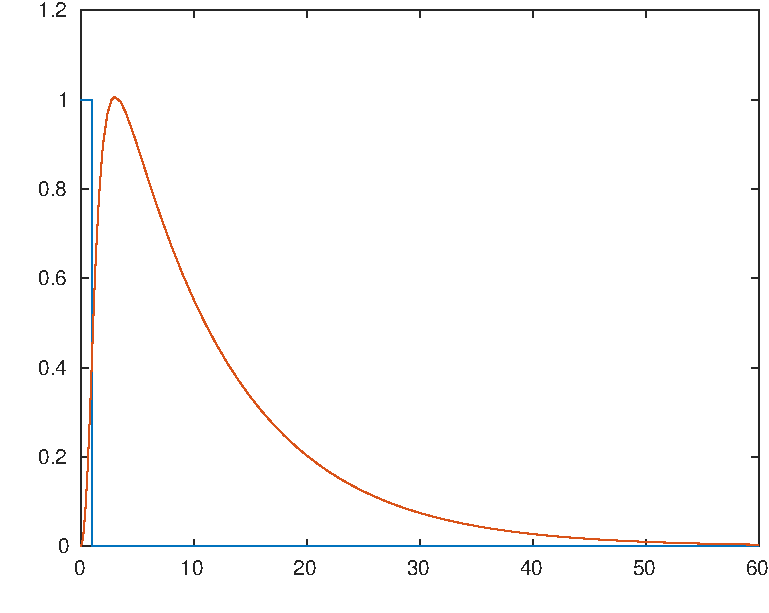
\includegraphics[width=\linewidth/2]{../Task1/ToReport/T1ImpulseResponse.pdf}\\
    \hbox to \linewidth {\hfil Step response \hfil Impulse response\hfil}\\
    
    \begin{center}
        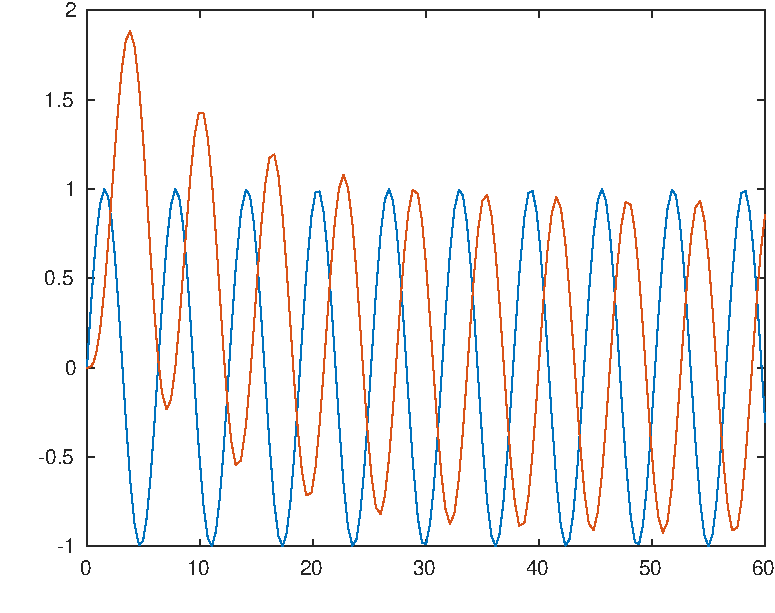
\includegraphics[width=\linewidth/2]{../Task1/ToReport/T1FreqResponse.pdf}\\
        Frequency response        
    \end{center}
    Note, that plots look like there is only one output, but it is not true -- 
    they are just very close to each other.

    \subsection*{C. Bode and Pole-Zero map plots}
    As a input signal, for which I will generate the plots I have chosen 
    a Frequency response (sine function).
    \begin{center}
        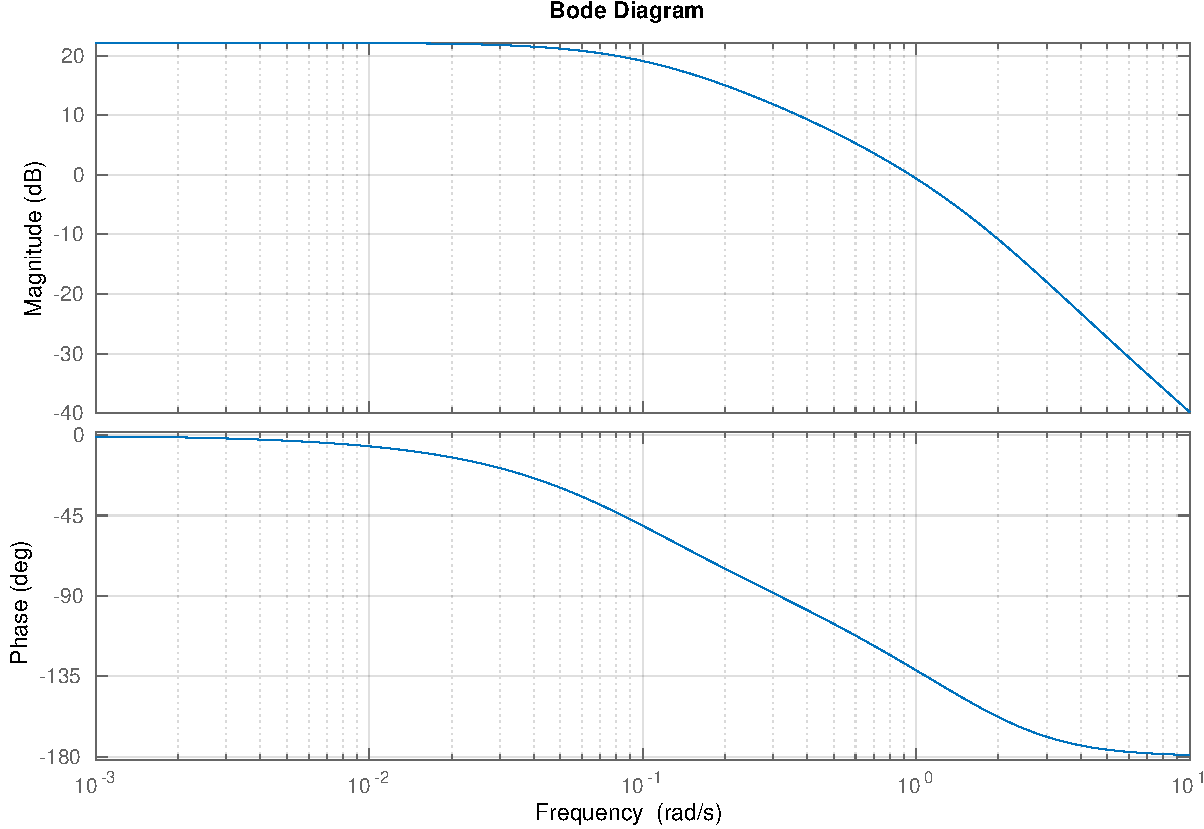
\includegraphics[width=\linewidth]{../Task1/ToReport/T1Bode.pdf}\\
        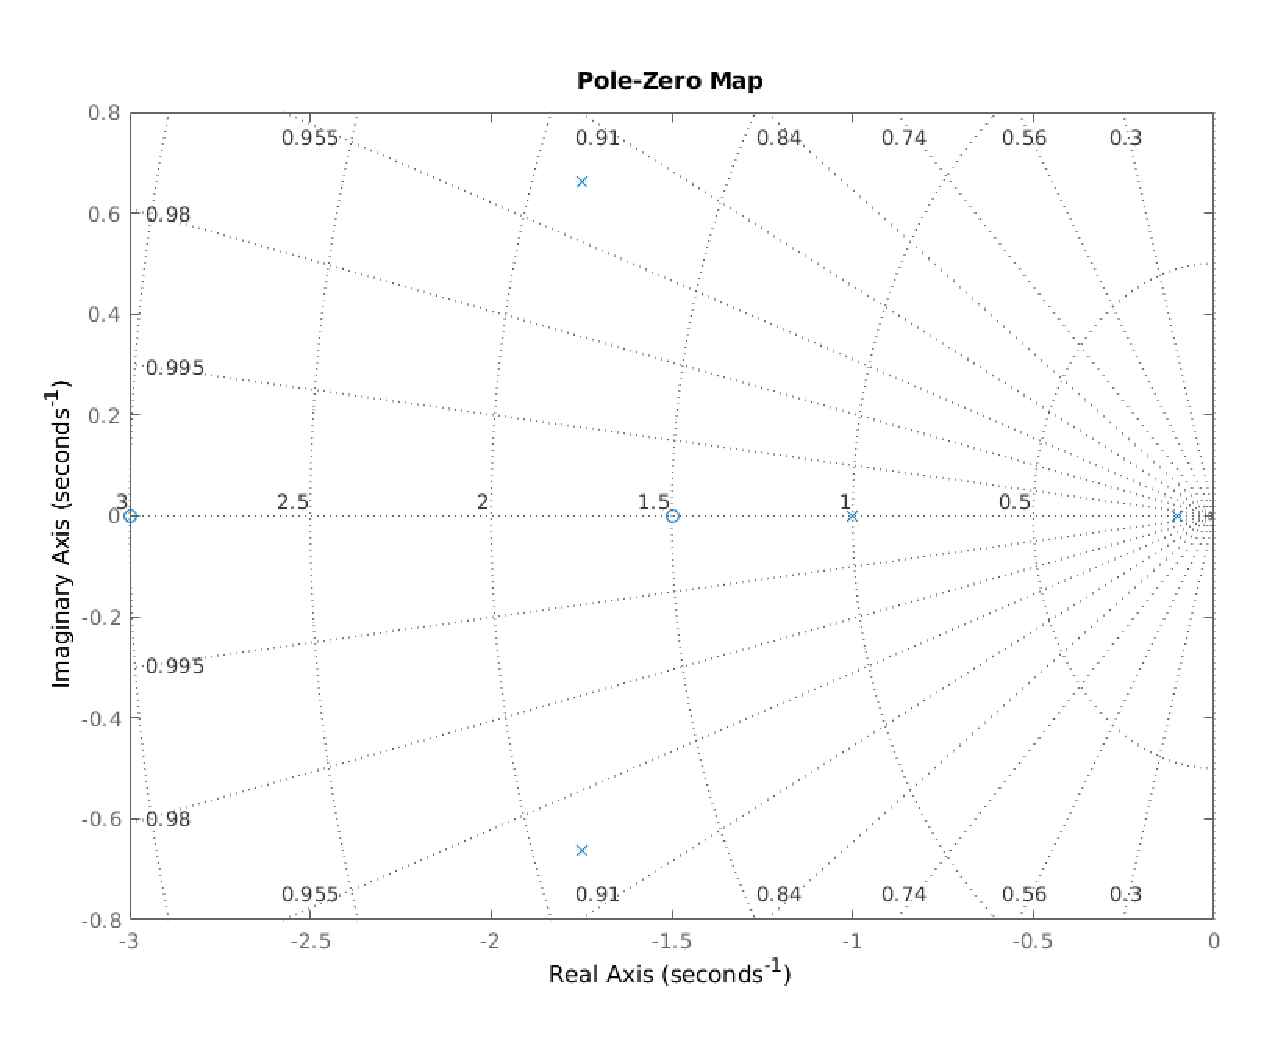
\includegraphics[width=\linewidth]{../Task1/ToReport/T1PoleZero.pdf}        
    \end{center}
    According to Matlab \texttt{pzmap()} function, our Transfer Function (1) has following poles 
    and zeroes:
    \begin{equation*}
    poles =
    \begin{bmatrix}
      -1.7500 + 0.6614i\\
      -1.7500 - 0.6614i\\
      -1.0000 + 0.0000i\\
      -0.1000 + 0.0000i
    \end{bmatrix} 
    zeroes =
    \begin{bmatrix}
        -3.0000\\
        -1.5000
    \end{bmatrix}
    \end{equation*}
    As it can be seen, all our poles have negative real part, and that says us 
    that the system is stable.
\newpage
\section{Task 2.}
    Find total Transfer Function of the system:
    \begin{center}
        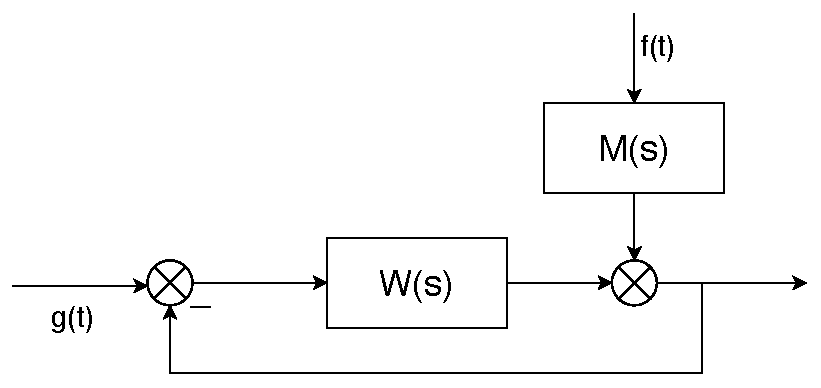
\includegraphics[scale=0.5]{../Task2/ToReport/System.pdf}
    \end{center}
    Firstly, let's consider case when $f(t)=0$. In this case our Transfer
    Function is $\frac{W}{1+W}$. Then we'll consider case, when $g(t)=0$, 
    and our Transfer Function will be $M \times \frac{1}{1+W}$.
    Hence, total transfer function for the system in general case is
    \begin{equation*}
        output = \frac{W}{1+W} \times g(t) + \frac{M}{1+W} \times f(t)
    \end{equation*}  
    In variant F I have:
    \begin{equation*}
    W(s) = \frac{s+1}{s^2+3s+2}, 
    M(s) = \frac{1}{s+3}
    \end{equation*}
    After simplification of fractions with Matlab, we get 
    \begin{equation*}
        output = \frac{1}{s+3} \times g(t) + \frac{s+1}{(s+3)^2 \times f(t)}
    \end{equation*}


\section{Used software.}
\begin{itemize}
    \item Python 3.8.1
    \item Matlab R2018b 9.5.0
    \item draw.io
\end{itemize}
All software was run under Manjaro Linux with 5.4.18-rt kernel
\end{document}